\chapter{Chapitre 3 : Déploiement, validation et conclusion}\label{chap7}

\section{Architecture de déploiement}

La Figure \ref{fig:deploy} présente la topologie des services. En local, Docker Compose orchestre la passerelle Nginx, le frontend React servi par Nginx, le backend Django sous Gunicorn, PostgreSQL, Redis, la chaîne Anvil, Fluent Bit, Elasticsearch et Kibana. Les healthchecks imposent l'ordre de démarrage : la base puis le backend, et enfin le frontend.

La cible d'exécution retient une base PostgreSQL managée (\textbf{RDS}) comme stockage par défaut et un \textbf{bucket S3} pour les fichiers médias. La configuration Django conserve le moteur PostgreSQL via les variables \texttt{DB\_*} et le backend de stockage via \texttt{STORAGE\_BACKEND}, ce qui rend le changement de service transparent pour le code applicatif.

\begin{figure}[H]
\centering
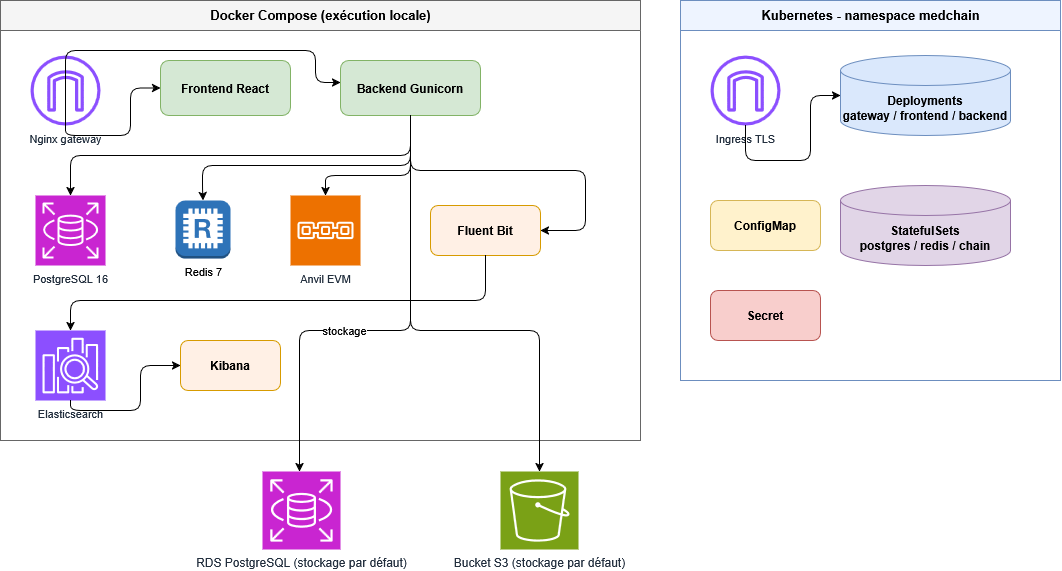
\includegraphics[width=\textwidth]{Chapters/7/images/03-topologie-deploiement.png}
\caption{Topologie de déploiement locale et cible}
\label{fig:deploy}
\end{figure}

\section{Conteneurisation et Kubernetes}

Chaque service possède image, variables d'environnement et healthcheck explicites. Les manifestes Kubernetes du namespace \texttt{medchain} complètent cette base avec un Ingress TLS, une ConfigMap, des Secrets, des volumes persistants et une séparation des composants de journalisation facultatifs.

\section{Validation fonctionnelle}

La validation a porté sur les points suivants :

\begin{itemize}
    \item construction des images backend et frontend ;
    \item connexion du backend à la base et exécution des migrations ;
    \item authentification d'un compte patient, d'un compte médecin et d'un compte administrateur ;
    \item appel d'une route protégée avec le jeton retourné ;
    \item vérification du filtrage des épisodes selon le rôle ;
    \item consultation de la timeline et des détails d'intégrité ;
    \item ancrage des blocs sur la chaîne locale et lecture des transactions ;
    \item service du frontend par la passerelle et accès à la documentation OpenAPI.
\end{itemize}

La Figure \ref{fig:swagger} illustre la documentation interactive générée automatiquement à partir du schéma OpenAPI.

\begin{figure}[H]
\centering
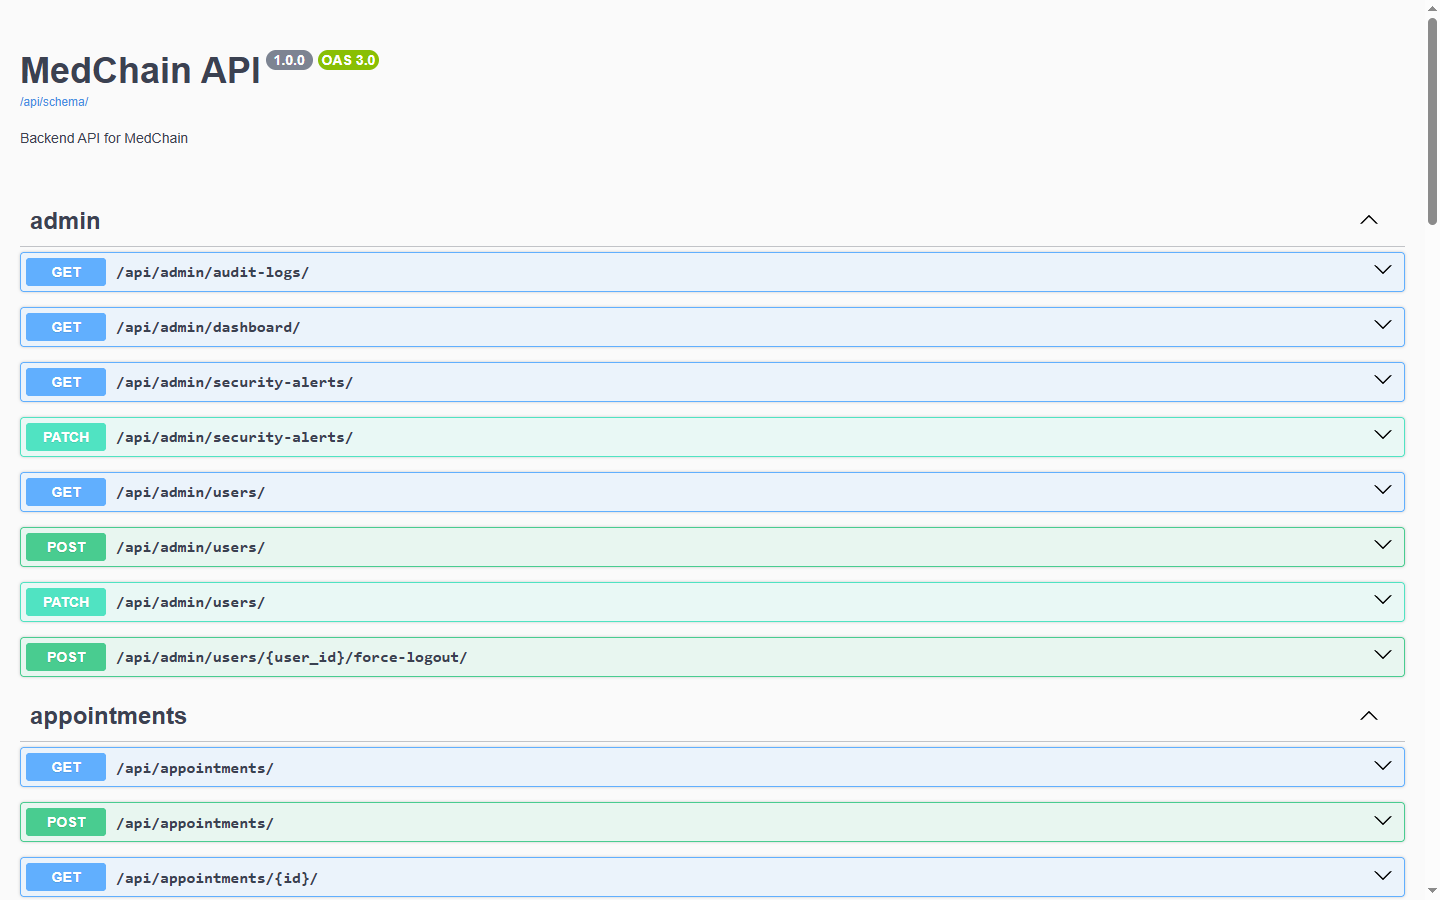
\includegraphics[width=\textwidth]{Images/Screenshots/S16-swagger-api.png}
\caption{Documentation interactive de l'API}
\label{fig:swagger}
\end{figure}

\section{Limites et perspectives}

Certaines évolutions restent à réaliser :

\begin{itemize}
    \item remplacer le fournisseur de clés basé sur l'environnement par un service de gestion de clés externe ;
    \item migrer l'ancrage local vers un registre public ou une infrastructure de production ;
    \item durcir les déploiements Kubernetes avec des politiques réseau et des quotas de ressources ;
    \item compléter la couverture de tests sur les scénarios d'accès refusé ;
    \item industrialiser le pipeline d'intégration continue avec analyse de sécurité des dépendances.
\end{itemize}

\section{Conclusion générale}

MedChain démontre qu'il est possible de concilier confidentialité et vérifiabilité dans un dossier médical partagé. Le chiffrement enveloppe protège le contenu, l'immutabilité des blocs et l'ancrage garantissent l'intégrité de l'historique, et le filtrage par rôle limite l'exposition des données. L'architecture conteneurisée et la séparation configuration/secrets fournissent une base pour un passage à l'échelle vers RDS et S3.
